\documentclass[12pt]{article}
\usepackage{amsmath, amssymb, amsthm, enumerate, graphicx}
\usepackage[usenames,dvipsnames]{color}
\usepackage{bm}
\usepackage[colorlinks=true,urlcolor=blue]{hyperref}
\usepackage{geometry}
\geometry{margin=1in}
\usepackage{float}
\usepackage{graphics}
\setlength{\marginparwidth}{2.15cm}
\usepackage{booktabs}
\usepackage{enumitem}
\usepackage{epsfig}
\usepackage{setspace}
\usepackage{parskip}
\usepackage[normalem]{ulem}
\usepackage{tikz}
\usetikzlibrary{positioning, arrows, automata}
\usepackage{pgfplots}
\usepackage[font=scriptsize]{subcaption}
\usepackage{float}
\usepackage[]{algorithm2e}
\usepackage{environ}
\usepackage{bbm}
\usepackage{graphicx}
\usepackage{titling}
\usepackage{url}
\usepackage{xcolor}
\usepackage{lipsum}
\usepackage{lastpage}
\usepackage[colorlinks=true,urlcolor=blue]{hyperref}
\usepackage{multicol}
\usepackage{tabularx}
\usepackage{comment}
\usepackage[utf8]{inputenc}
\usepackage{amssymb}
\usepackage{setspace}
\usepackage{marvosym}
\usepackage{wrapfig}
\usepackage{datetime}
\usepackage[many]{tcolorbox}
\usepackage{array}
\usepackage{multirow}
\usepackage{wasysym}
\usepackage{cancel}
\usepackage{float}
\usepackage{listings}
\usepackage{color}
\usepackage[thinlines]{easytable}
\usepackage{booktabs}
\usepackage{rotating}

\newcommand{\R}{\mathbb{R}}
\newcommand{\blackcircle}{\tikz\draw[black,fill=black] (0,0) circle (1ex);}
\renewcommand{\circle}{\tikz\draw[black] (0,0) circle (1ex);}


%\newcommand{\norm}[1]{\lVert #1 \rVert}
%\newcommand{\st}{\mathrm{s.t.}}

\makeatletter
\newcommand{\removelatexerror}{\let\@latex@error\@gobble}
\makeatother

\newcommand{\argmax}{\mathop{\mathrm{argmax}}}
\newcommand{\argmin}{\mathop{\mathrm{argmin}}}


%%%%%%%%%%%%%%%%%%%%%%%%%%%%%%%%%%%%%%%%%%%
% Custom box for highlights               %
%%%%%%%%%%%%%%%%%%%%%%%%%%%%%%%%%%%%%%%%%%%

% Define box and box title style
\tikzstyle{mybox} = [fill=blue!10, very thick,
    rectangle, rounded corners, inner sep=1em, inner ysep=1em]

% \newcommand{\notebox}[1]{
% \begin{tikzpicture}
% \node [mybox] (box){%
%     \begin{minipage}{\textwidth}
%     #1
%     \end{minipage}
% };
% \end{tikzpicture}%
% }

\NewEnviron{notebox}{

\begin{tikzpicture}
\node [mybox] (box){
    \begin{minipage}{\textwidth}
        \BODY
    \end{minipage}
};
\end{tikzpicture}
}
\begin{document}

\section*{}
\begin{center}
  \centerline{\textsc{\LARGE  Homework 2 Template (v1, released Oct. 1st)}}
\end{center}

Enter your team's andrew IDs in the boxes below.  If you do not do this, you may lose points on your assignment.

AndrewId 1: \begin{tcolorbox}[fit,height=1cm, width=5cm, blank, borderline={1pt}{1pt},nobeforeafter]
    \begin{center}
    \vspace{3mm}
    ielshar
    \end{center}
\end{tcolorbox}
    \\
AndrewId 2: \begin{tcolorbox}[fit,height=1cm, width=5cm, blank, borderline={1pt}{1pt},nobeforeafter]
    \begin{center}
    \vspace{3mm}
    mharding
    \end{center}
\end{tcolorbox} \\
\vspace{0.5cm}

Use this template to record your answers for Homework 2.  Add your answers using LaTeX and then save your document as a pdf to upload to gradescope.  You are required to use this template to submit your answers.  \textbf{You should not alter this template in any way} other than to insert your solutions.  You must submit all 13 pages of this template to gradescope.  Do not remove the instructions page(s).  Altering this template or including your solutions outside of the provided boxes can result in your assignment being graded incorrectly.  You may lose points if you do not follow these instructions.

\section*{Instructions for Specific Problem Types}

% For ``Select One" questions, please use a ``filled in'' circle to indicate your answer:

% \begin{quote}
% \textbf{Select One:} Which of these is an instructor of this course?
% \begin{list}{}
%      \item\CIRCLE{} Tom Mitchell
%      \item\Circle{} Marie Curie
%      \item\Circle{} Noam Chomsky
% \end{list}
% \end{quote}

For questions where you must fill in a blank, please make sure your final answer is fully included in the given space.  \textbf{Do not change the size of the box provided.}  For short answer questions you should \textbf{not} include your work in your solution.  Only provide an explanation or proof if specifically asked.  Otherwise, your assignment may not be graded correctly, and points may be deducted from your assignment.

\begin{quote}
\textbf{Fill in the blank:} What is the course number?

\begin{tcolorbox}[fit,height=1cm, width=4cm, blank, borderline={1pt}{-2pt},nobeforeafter]
    \begin{center}\huge10-703\end{center}
    \end{tcolorbox}
\end{quote}


\newpage
\section*{Question 1 Convolutional Neural Network}
\subsection*{Question 1.a}
    \qquad 
    \textbf{y} =  \begin{tcolorbox}[fit,height=1cm, width=6cm, blank, borderline={1pt}{1pt},nobeforeafter]
            \begin{center}
            \vspace{3mm}
            [4, -3]
            \end{center}
            \end{tcolorbox}
\subsection*{Question 1.b}
\begin{enumerate}
        \item{loss value using original weights: }
            \begin{tcolorbox}[fit,height=1cm, width=2cm, blank, borderline={1pt}{1pt},nobeforeafter]
            \begin{center}
            \vspace{3mm}
            37
            \end{center}
            \end{tcolorbox} \vspace{0.8cm} \\
        \item{new weights} 
            \begin{tcolorbox}[fit,height=1cm, width=9cm, blank, borderline={1pt}{1pt},nobeforeafter]
            \begin{center}
            \vspace{3mm}
            [0.72, 0.34, -0.84]
            \end{center}
            \end{tcolorbox}
            \vspace{0.8cm} \\
        \item{output using new weights}
            \begin{tcolorbox}[fit,height=1cm, width=6cm, blank, borderline={1pt}{1pt},nobeforeafter]
            \begin{center}
            \vspace{3mm}
            [3.36, -1.36]
            \end{center}
            \end{tcolorbox}
            \vspace{0.8cm} \\
        \item{loss using new weights}
            \begin{tcolorbox}[fit,height=1cm, width=2cm, blank, borderline={1pt}{1pt},nobeforeafter]
            \begin{center}
            \vspace{3mm}
            19.1392
            \end{center}
            \end{tcolorbox}
\end{enumerate}

\newpage
\section*{Question 2 Policy Iteration and Value Iteration}
    \begin{tcolorbox}[fit,height=8cm, width=\textwidth, blank, borderline={1pt}{-2pt},nobeforeafter]
    Policy iteration and Value Iteration algorithms have guaranteed convergence due critically to the Gamma contraction maaping property of the tabular Bellman update operation. In other words, in finite MDPs, a Bellman update operation on any value function will monotonically improve the value function, which in turn can be used to create an improved policy. However, if a function approximator for V($s$) or Q($s,a$) such as a neural network is used instead of this finite tabular representation, then we lose the Gamma contraction mapping property of the approximator updates. This is because an exact Bellman update operation may not be performed on the function approximator as there are no guarantees od convergence or the neural network might even diverge, and therefore the updates cannot be guaranteed to strictly improve the Value or Q-value functions.
    \end{tcolorbox}
\newpage
\section*{Question 3 Continuation Function}
\subsection*{Question 3.a}
\begin{enumerate}
    \item{Derive the recurrence relation} \vspace{4pt} \\
    \begin{tcolorbox}[fit,height=12cm, width=\textwidth, blank, borderline={1pt}{-2pt},nobeforeafter]
    \begin{align}
    C(s_1,a_1) & = \gamma\sum_{s_2}T(s_1,a_1,s_2)\cdot V(s_2)\\
    & =  \gamma\sum_{s_2}T(s_1,a_1,s_2) \cdot \max_{a_2} ( R(s_2, a_2) + C(s_2, a_2))
    \end{align}
    (2) follows (1) as we can show that:
    \begin{align}
    V(s_2) & = \max_{a_2} \left( R(s_2,a_2) + \gamma \sum_{s_3}T(s_2, a_2, s_3)V(s_3) \right)\\
    & = \max_{a_2} \left( R(s_2,a_2) + C(s_2,a_2) \right)
    \end{align}

    \end{tcolorbox}
   \item{Fill in the table} \vspace{4pt} \\
   \begin{enumerate}[label=\roman*)]
        \item \qquad
            \begin{tcolorbox}[fit,height=3cm, width=12cm, blank, borderline={1pt}{1pt},nobeforeafter]
            \begin{center}
            \vspace{3mm}
            $$ V(s) = \max_{a} (R(s,a) + C(s,a))$$
            \end{center}
            \end{tcolorbox}
        \item \qquad
            \begin{tcolorbox}[fit,height=3cm, width=12cm, blank, borderline={1pt}{1pt},nobeforeafter]
            \begin{center}
            \vspace{3mm}
            $$ Q(s, a) = R(s,a) + \gamma\sum_{s'}T(s,a,s')\cdot V(s') $$
            \end{center}
            \end{tcolorbox}
        \item \qquad
        \begin{tcolorbox}[fit,height=3cm, width=12cm, blank, borderline={1pt}{1pt},nobeforeafter]
            \begin{center}
            \vspace{3mm}
            $$ Q(s,a) = R(s,a) + C(s,a) $$
            \end{center}
            \end{tcolorbox}
        \item \qquad
            \begin{tcolorbox}[fit,height=3cm, width=12cm, blank, borderline={1pt}{1pt},nobeforeafter]
            \begin{center}
            \vspace{3mm}
            $$ C(s,a) = \gamma\sum_{s'}T(s,a,s')\max_{a'}Q(s',a') $$
            \end{center}
            \end{tcolorbox}
    \end{enumerate}
\end{enumerate}
\subsection*{Question 3.b}
\begin{enumerate}
    \item 
    \begin{tcolorbox}[fit,height=4cm, width=\textwidth, blank, borderline={1pt}{-2pt},nobeforeafter]
    True, knowing $Q(s,a)$ is better than knowing $V(s)$ if we don't know $T, R$ because $Q(s,a)$ captures all necessary information from $T$ and $R$, %, and choosing optimal actions' values from $Q(s,a)$ can be used to compute $V(s)$ like: $V(s) = \max_aQ(s,a)$.
    since $\pi^*(s)=\argmax_a(Q(s,a))$ but if we use $V(s)$ to compute the optimal action we need to know $T(s,a,s')$ since  $\pi^*(s)=\argmax_a(R(s,a)+\gamma\sum_{s'}T(s,a,s') V(s'))$.
    \end{tcolorbox}
    \item 
    \begin{tcolorbox}[fit,height=4cm, width=\textwidth, blank, borderline={1pt}{-2pt},nobeforeafter]
    False, knowing $C(s,a)$ is better because it captures $T$ and we only need to know $R(s,a)$ whereas $V(s)$ still needs $T$ to compute state values and that information about $T$ is lacking. $\pi^*(s)$ can be computed using only $\pi^*(s) = \argmax_a ( R(s,a) + C(s,a))$.
    \end{tcolorbox}
\end{enumerate}


\newpage
\section*{Question 4 Importance Sampling}
\begin{enumerate}
     \item 
        Expectation: \begin{tcolorbox}[fit,height=1cm, width=3cm, blank, borderline={1pt}{1pt},nobeforeafter]
        \begin{center}
        \vspace{3mm}
        0.8 
        \end{center}
        \end{tcolorbox} \vspace{5mm}\\
        Variance: \hspace{0.47cm} \begin{tcolorbox}[fit,height=1cm, width=3cm, blank, borderline={1pt}{1pt},nobeforeafter]
            \begin{center}
            \vspace{3mm}
            0.774286 
            \end{center}
            \end{tcolorbox}  
    \item Direct Sampling \vspace{0.3cm} \\
    \begin{tcolorbox}[fit,height=10cm, width=\textwidth, blank, borderline={1pt}{-2pt},nobeforeafter]
For 10 samples, expected value and variance: 0.5175211497062785 0.22445729082239635\\
For 1000 samples, expected value and variance: 0.7801754107151546 0.7679549069879695\\
For 10k samples, expected value and variance: 0.7900644740717525 0.764102137090607\\\\
		By the strong law of large numbers the as the number of samples increases, the sample mean and variance converges a.s to $\mathbf{E}_{~p}[f(x)]$ and ${\rm Var}(f(x))$ (seed used: 10703)\\
    \end{tcolorbox}
    \newpage 
    \item Importance Sampling \vspace{0.3cm} \\
    \begin{tcolorbox}[fit,height=10cm, width=\textwidth, blank, borderline={1pt}{-2pt},nobeforeafter]
    Q(x) = norm(3,1):\\
For 10 samples, expected value and variance: 4.295353386364986 166.05054642381438\\
For 1000 samples, expected value and variance: 1.2630579295295916 55.00040929485666\\
For 10k samples, expected value and variance: 0.8143918731813137 34.32446852702005\\
Q(x) = norm(0,1):\\
For 10 samples, expected value and variance: 0.35818306780353104 0.49598389429460665\\
For 1000 samples, expected value and variance: 0.7440814888529712 3.703013244355498\\
For 10k samples, expected value and variance: 0.7658318235847844 3.9772672572375267\\
Q(x) = $15/16\cdot x^2 \cdot (1+x)^2$:\\
For 10 samples, expected value and variance: 0.7999999999999999 8.628166150854816e-33\\
For 1000 samples, expected value and variance: 0.8000000000000002 3.4944072910962007e-32\\
For 10k samples, expected value and variance: 0.8 1.1985755378701749e-32 \\
(seed used: 10703)\\

The proposal distribution $q(x) = 15/16x^2\cdot (1+x)^2$ gives the lowest variance. This is because its support of values is the same as that of $p(x)$, i.e. $-1 \le x \le 1$ and the ratio of $p(x)/q_3(x)$ when multiplied with $f(x)$ equals a constant: $p(x)/q_3(x) \cdot f(x) = 4/5$. Therefore, the variance of $p/q_3\cdot f$ must aprox. 0 using importance sampling from proposal distribution $q_3$. The $q_1 = N(3,1)$ proposal distribution converges the slowest because it samples most often outside the range $-1 \le x \le 1$  of $p(x)$ since its mean is 3. Many samples were needed to inform the sample mean and sample variance about samples of $f(x)$ within the range of $p$.
    \end{tcolorbox}
    
    \item Weighted Importance Sampling \vspace{0.3cm}\\
    \begin{tcolorbox}[fit,height=10cm, width=\textwidth, blank, borderline={1pt}{-2pt},nobeforeafter]
    Q(x) = norm(3,1):\\
For 10 samples, expected value and variance: 1.65367501514988 \\
For 1000 samples, expected value and variance: 0.6347482121569935 \\
For 10k samples, expected value and variance: 0.8159765021680583 \\
Q(x) = norm(0,1):\\
For 10 samples, expected value and variance: 0.5678804940372946 \\
For 1000 samples, expected value and variance: 0.750091065121246 \\
For 10k samples, expected value and variance: 0.7790952791280585 \\
Q(x) = $15/16*x^2*(1+x)^2$:\\
For 10 samples, expected value and variance: 1.7487719726369466 \\
For 1000 samples, expected value and variance: 0.9252790478202617 \\
For 10k samples, expected value and variance: 0.8969532357821838 \\
(seed used: 10703)\\

In the weighted importance sampling, we see that the sample mean approaches a different value than importance sampling did. Weighted importance sampling is a biased estimator.
    \end{tcolorbox}
\end{enumerate}
\newpage 
\section*{Question 5 MC and TD Methods}
\begin{enumerate}
    \item 
        S0: \begin{tcolorbox}[fit,height=1cm, width=2cm, blank, borderline={1pt}{1pt},nobeforeafter]
        \begin{center}
        \vspace{3mm}
        5
        \end{center}
        \end{tcolorbox}
        \qquad
        S1: \begin{tcolorbox}[fit,height=1cm, width=2cm, blank, borderline={1pt}{1pt},nobeforeafter]
        \begin{center}
        \vspace{3mm}
        25
        \end{center}
        \end{tcolorbox}
        \qquad
        S2: \begin{tcolorbox}[fit,height=1cm, width=2cm, blank, borderline={1pt}{1pt},nobeforeafter]
        \begin{center}
        \vspace{3mm}
        20
        \end{center}
        \end{tcolorbox}
        \qquad
        S3: \begin{tcolorbox}[fit,height=1cm, width=2cm, blank, borderline={1pt}{1pt},nobeforeafter]
        \begin{center}
        \vspace{3mm}
        17
        \end{center}
        \end{tcolorbox} \vspace{0.8cm} \\
        S4: \begin{tcolorbox}[fit,height=1cm, width=2cm, blank, borderline={1pt}{1pt},nobeforeafter]
        \begin{center}
        \vspace{3mm}
        5
        \end{center}
        \end{tcolorbox}
        \qquad
        S5: \begin{tcolorbox}[fit,height=1cm, width=2cm, blank, borderline={1pt}{1pt},nobeforeafter]
        \begin{center}
        \vspace{3mm}
        -5
        \end{center}
        \end{tcolorbox}
        \qquad
        S6: \begin{tcolorbox}[fit,height=1cm, width=2cm, blank, borderline={1pt}{1pt},nobeforeafter]
        \begin{center}
        \vspace{3mm}
        -5
        \end{center}
        \end{tcolorbox}
        \qquad
        \vspace{1cm}
    \item 
        S0: \begin{tcolorbox}[fit,height=1cm, width=2cm, blank, borderline={1pt}{1pt},nobeforeafter]
        \begin{center}
        \vspace{3mm}
       20
        \end{center}
        \end{tcolorbox}
        \qquad
        S1: \begin{tcolorbox}[fit,height=1cm, width=2cm, blank, borderline={1pt}{1pt},nobeforeafter]
        \begin{center}
        \vspace{3mm}
        23
        \end{center}
        \end{tcolorbox}
        \qquad
        S2: \begin{tcolorbox}[fit,height=1cm, width=2cm, blank, borderline={1pt}{1pt},nobeforeafter]
        \begin{center}
        \vspace{3mm}
        21
        \end{center}
        \end{tcolorbox}
        \qquad
        S3: \begin{tcolorbox}[fit,height=1cm, width=2cm, blank, borderline={1pt}{1pt},nobeforeafter]
        \begin{center}
        \vspace{3mm}
        28
        \end{center}
        \end{tcolorbox} \vspace{0.8cm} \\
        S4: \begin{tcolorbox}[fit,height=1cm, width=2cm, blank, borderline={1pt}{1pt},nobeforeafter]
        \begin{center}
        \vspace{3mm}
        31
        \end{center}
        \end{tcolorbox}
        \qquad
        S5: \begin{tcolorbox}[fit,height=1cm, width=2cm, blank, borderline={1pt}{1pt},nobeforeafter]
        \begin{center}
        \vspace{3mm}
        23
        \end{center}
        \end{tcolorbox}
        \qquad
        S6: \begin{tcolorbox}[fit,height=1cm, width=2cm, blank, borderline={1pt}{1pt},nobeforeafter]
        \begin{center}
        \vspace{3mm}
        13
        \end{center}
        \end{tcolorbox}
        \qquad
        \vspace{1cm}
    \item 
        S0: \begin{tcolorbox}[fit,height=1cm, width=2cm, blank, borderline={1pt}{1pt},nobeforeafter]
        \begin{center}
        \vspace{3mm}
        25.296875
        \end{center}
        \end{tcolorbox}
        \qquad
        S1: \begin{tcolorbox}[fit,height=1cm, width=2cm, blank, borderline={1pt}{1pt},nobeforeafter]
        \begin{center}
        \vspace{3mm}
        28.59375
        \end{center}
        \end{tcolorbox}
        \qquad
        S2: \begin{tcolorbox}[fit,height=1cm, width=2cm, blank, borderline={1pt}{1pt},nobeforeafter]
        \begin{center}
        \vspace{3mm}
        29.1875
        \end{center}
        \end{tcolorbox}
        \qquad
        S3: \begin{tcolorbox}[fit,height=1cm, width=2cm, blank, borderline={1pt}{1pt},nobeforeafter]
        \begin{center}
        \vspace{3mm}
        32.375
        \end{center}
        \end{tcolorbox} \vspace{0.8cm} \\

        S4: \begin{tcolorbox}[fit,height=1cm, width=2cm, blank, borderline={1pt}{1pt},nobeforeafter]
        \begin{center}
        \vspace{3mm}
        29.75
        \end{center}
        \end{tcolorbox}
        \qquad
        S5: \begin{tcolorbox}[fit,height=1cm, width=2cm, blank, borderline={1pt}{1pt},nobeforeafter]
        \begin{center}
        \vspace{3mm}
        20.5
        \end{center}
        \end{tcolorbox}
        \qquad
        S6: \begin{tcolorbox}[fit,height=1cm, width=2cm, blank, borderline={1pt}{1pt},nobeforeafter]
        \begin{center}
        \vspace{3mm}
        13
        \end{center}
        \end{tcolorbox}
        \qquad
\end{enumerate}

\newpage
\section*{Question 6 Programming Question}
    \begin{tcolorbox}[fit,height=22cm, width=\textwidth, blank, borderline={1pt}{-2pt},nobeforeafter]
    {\large 6.1, 6.2, 6.3 (a)}\\
    {\large *Dueling architecture's 2 streams were merged using equation (9) from [4]. For MountainCar-v0 environment, the value and advantage stream shared the 3rd hidden layer of a DQN network in order to not thin out the backprop gradient over a fork in the network (*motivated by TA Nicholay Topkin). As well, for both DQN and Dueling networks, a periodically heldout target model was used to compute the target values in the objective. DDQN learned using 2 DQN networks, updated symmetrically, as described in [3]. All networks were trained using mean-squared-error objective over minibatches.}
	\begin{table}[H]
		\centering
		\caption{Implementation settings}
		\begin{tabular}{|c|p{7.785em}|l|l|r|}
			\cline{2-5}    \multicolumn{1}{r|}{} & Settings & \multicolumn{1}{p{7.93em}|}{DQN} & \multicolumn{1}{p{7.93em}|}{DDQN} & \multicolumn{1}{p{7.5em}|}{Dueling} \\
			\hline
			\multirow{10}[20]{*}{\begin{sideways}CartPole-v0\end{sideways}} & NN MLP Architecture  & \multicolumn{1}{p{7.93em}|}{2 hidden layers each of size 32 with relu activation} & \multicolumn{1}{p{7.93em}|}{2 hidden layers each of size 60 with relu activation} & \multicolumn{1}{p{7.93em}|}{2 streams with 1 relu hidden layer of size 128 each connected to 1 shared hidden layer of size 64 with relu, merged according to (9) from [4], (see HW refs).} \\
			\cline{2-5}          & optimizer & \multicolumn{1}{p{7.93em}|}{Adam} & \multicolumn{1}{p{7.93em}|}{Adam} & \multicolumn{1}{p{7.93em}|}{Adam} \\
			\cline{2-5}          & Burn-in transitions & 10000 & 10000 &  10000 \\
			\cline{2-5}          & Initial epsilon & 0.5   & 1     & 0.5 \\
			\cline{2-5}          & Final epsilon & 0.1   & 0.1   & 0.1 \\
			\cline{2-5}          & Exploration decay steps & \multicolumn{1}{p{7.93em}|}{$2\times10^5$} & \multicolumn{1}{p{7.93em}|}{$2\times10^5$} & \multicolumn{1}{p{7.93em}|}{$5\times10^4$} \\
			\cline{2-5}          & minibatch size & 32    & 32    & 32  \\
			\cline{2-5}          & no. of steps until target network is updated & 100   & 100   & 100  \\
			\cline{2-5}          & steps before minibatch & 4     & 1     & 4 \\
			\cline{2-5}          & learning rate & 0.0001 & 0.0001 &  0.0001 \\
			\hline
			\multirow{10}[20]{*}{\begin{sideways}MountainCar-v0\end{sideways}} & NN MLP Architecture  & \multicolumn{1}{p{7.93em}|}{3 hidden layers each of size 60 with relu activation} & \multicolumn{1}{p{7.93em}|}{3 hidden layers each of size 60 with relu activation} & \multicolumn{1}{p{7.93em}|}{2 streams with 1 linear hidden layer of size 64 each placed ontop of 3 hidden relu layers of size 64 each, then merged using (9) as above.} \\
			\cline{2-5}          & optimizer & \multicolumn{1}{p{7.93em}|}{Adam} & \multicolumn{1}{p{7.93em}|}{Adam} & \multicolumn{1}{p{7.93em}|}{Adam} \\
			\cline{2-5}          & Burn-in transitions & 10000 & 10000 & 10000 \\
			\cline{2-5}          & Initial epsilon & 0.5   & 1     & 0.5  \\
			\cline{2-5}          & Final epsilon & 0.1   & 0.1   &  0.1 \\
			\cline{2-5}          & Exploration decay steps & \multicolumn{1}{p{7.93em}|}{$2\times10^5$} & \multicolumn{1}{p{7.93em}|}{$2\times10^5$} & \multicolumn{1}{p{7.93em}|}{$2\times10^6$} \\
			\cline{2-5}          & minibatch size & 32    & 32    & 32 \\
			\cline{2-5}          & no. of steps until target network is updated & 100   & 100   & 16 \\
			\cline{2-5}          & steps before minibatch & 4     & 4     & 4 \\
			\cline{2-5}          & learning rate & 0.0001 & 0.00007 & 0.0004 \\
			\hline
		\end{tabular}%
		\label{tab1}%
	\end{table}%
     
    \end{tcolorbox}
    \begin{tcolorbox}[fit,height=22cm, width=\textwidth, blank, borderline={1pt}{-2pt},nobeforeafter]
    {\large 6.1 (b) and (c)} \\
    {\large CartPole-v0 DQN training and performace plots:} \\
    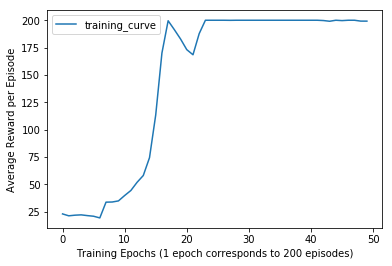
\includegraphics[width=.5\textwidth]{figures/CP_dqn_training_curve}
    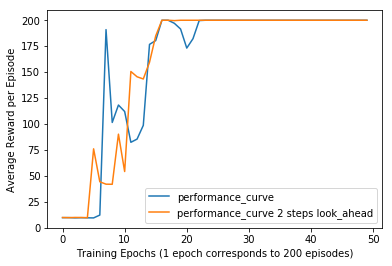
\includegraphics[width=.5\textwidth]{figures/CP_dqn_performance_curve}
    The training curve shows that our agent have learned to perform optimally in CartPole after about 25 epochs where it is stabilized there after. \\
    The performance curves show that the two step look ahead policy performes better than the greedy policy w.r.t Q, where Q is learned from DQN, this result is expected, except at some point around 10 epochs in the training. This could be due to the fact the agent haven't learned Q values close to the true Q values just yet, we see however that this behavior is no longer the case after around 20 epochs where Q has converged to the true values.\\
    \\
    {\large Mountaincar-v0 DQN training and performace plots:} \\
    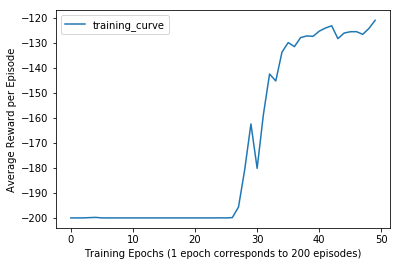
\includegraphics[width=.5\textwidth]{figures/MC_dqn_training_curve}
    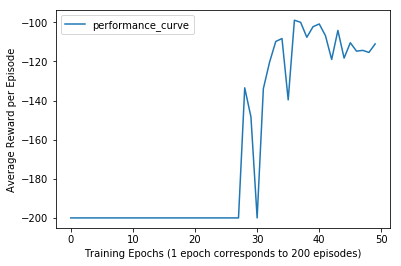
\includegraphics[width=.5\textwidth]{figures/MC_dqn_performance_curve}
	The training curve shows that our agent took about 27 training epochs in order to learn the Q value that induce a policy that reaches the flag in Mountain Car. The reason behind this could be due to the fact that Mountain car is a harder environment than cartPole since a random policy which we start with is highly unlikely to reach the flag. This problem could be mitigated by having the NN model predict initially Q values that are some how optimitic. The training curve seems to have converged to average values between -130 and -120 at the end training (min $\epsilon=0.1$ is reached), which is pretty good for this environment.  \\
	The performance curves using $\epsilon$-greedy policy ($\epsilon$=0.05) is consistent with the training curve. The average reward per episode seems to be around -115 near the end of training.   \\
	{\large 6.1 (d):} please refer to the submitted videos. \\
	{\large 6.1 (e):} The below table was generated using a \textbf{greedy} policy. The results shows that our agent was able to pass all episodes with max reward for CartPole and performs very well with $  $MountainCar (can reach the flag by approx. 110 steps on avg.).
	\vspace*{-0.6cm}
    \begin{table}[H]
	\centering
	\caption{ \small DQN: Avg. total reward per 100 episode +/- std.}
	\vspace*{-0.3cm}
	\begin{tabular}{|p{13em}|r|}
		\hline
		\textbf{\footnotesize Setting} & \multicolumn{1}{p{10.645em}|}{\textbf{ \footnotesize mean $\pm$ std.}} \\
		\hline
		{\footnotesize CartPole DQN} & \multicolumn{1}{l|}{200.0 $\pm$ 0.0} \\
		\hline
		{\footnotesize CartPole DQN 2-step LA} & \multicolumn{1}{l|}{200.0 $\pm$ 0.0} \\
		\hline
		{\footnotesize MountainCar DQN} & \multicolumn{1}{l|}{-109.85 $\pm$ 11.6115} \\
		\hline
	\end{tabular}%
	\label{tabDQN}%
	\end{table}%    
	

	
	
    \end{tcolorbox}
    \begin{tcolorbox}[fit,height=22cm, width=\textwidth, blank, borderline={1pt}{-2pt},nobeforeafter]
    {\large 6.2  (b) and (c)} \\
    {\large CartPole-v0 DDQN training and performace plots:} \\
    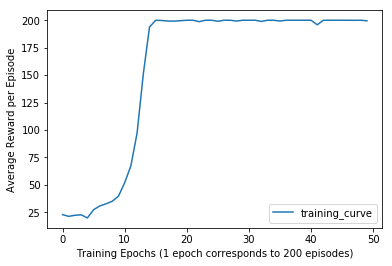
\includegraphics[width=.5\textwidth]{figures/CP_ddqn_training_curve}
    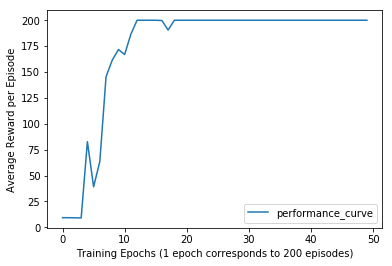
\includegraphics[width=.5\textwidth]{figures/CP_ddqn_performance_curve}
    The training curve for DDQN shows that our agent have learned to perform optimally in CartPole after about 15 epochs where it is stabilized there after. \\
    The performance curve shows that the agent have learnt to act optimally where the average reward achieved per episode after 20 epochs is the maximum achievable.\\
    Compared to DQN, DDQN performs consistently better since it solves the Q-values overestimation problem of DQN. Dueling converges quicker than DDQN for this environment, however, DDQN has more robust performance after convergence.
    \\
   	{\large Mountaincar-v0 DDQN training and performace plots:} \\
    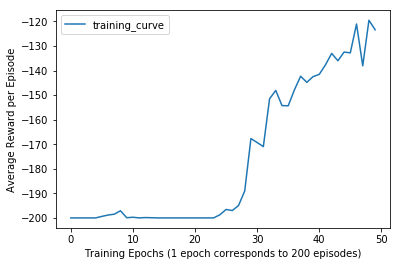
\includegraphics[width=.5\textwidth]{figures/MC_ddqn_training_curve}
    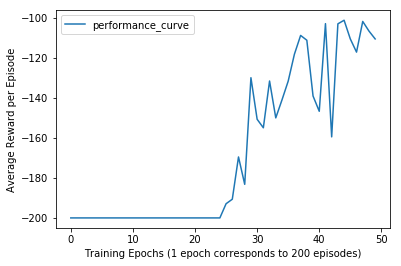
\includegraphics[width=.5\textwidth]{figures/MC_ddqn_performance_curve}
   	The training curve for DDQN shows that our agent took about 24 training epochs in order to learn the Q values that induce a policy that reaches the flag in Mountain Car. It also shows that our agent is learning consistently overtime where the avg. reward per episode hits -120 towards the end of training. It is worth mentioning that in our case finding the right hyperparameters for the DDQN to achieve this performance in MountainCar was not an easy task.  \\
    The performance curves using $\epsilon$-greedy policy ($\epsilon$=0.05) is consistent with the training curve. The average reward per episode seems to be around -115 on average near the end of training.   \\
    DDQN seems to have less effect w.r.t DQN results on this environment the reason may be that fact that it was harder for us to find the best parameters for DDQN. Perhaps better results could be achieved with more parameter tweaking.\\
    {\large 6.1 (d):} please refer to the submitted videos. \\
    {\large 6.1 (e):} The below table was generated using a \textbf{greedy} policy. The results shows that our agent was able to pass all episodes with max reward for CartPole and performs very well with $  $MountainCar (can reach the flag by approx. 108 steps on avg.). Note that the mean and std. for MountainCar are better than that of DQN.
    \vspace*{-0.6cm}
      \begin{table}[H]
    	\centering
    	\caption{ \footnotesize DDQN: Avg. total reward per 100 episode +/- std.}
    	\vspace*{-0.4cm}
    	\begin{tabular}{|p{9.43em}|r|}
    		\hline
    		\textbf{\footnotesize Setting} & \multicolumn{1}{p{10.645em}|}{\textbf{ \footnotesize mean $\pm$ std.}} \\
    		\hline
    		{\footnotesize CartPole DDQN} & \multicolumn{1}{l|}{\footnotesize 200.0 $\pm$ 0.0} \\
    		\hline
    		{\footnotesize MountainCar DDQN} & \multicolumn{1}{l|}{\footnotesize -108.59 $\pm$ 9.8347} \\
    		\hline
    	\end{tabular}%
    	\label{tabDDQN}%
    \end{table}%
    \end{tcolorbox}
    \begin{tcolorbox}[fit,height=22cm, width=\textwidth, blank, borderline={1pt}{-2pt},nobeforeafter]
    {\large 6.3  (b) and (c)} \\
    {\large CartPole-v0 Dueling training and performace plots:} \\
    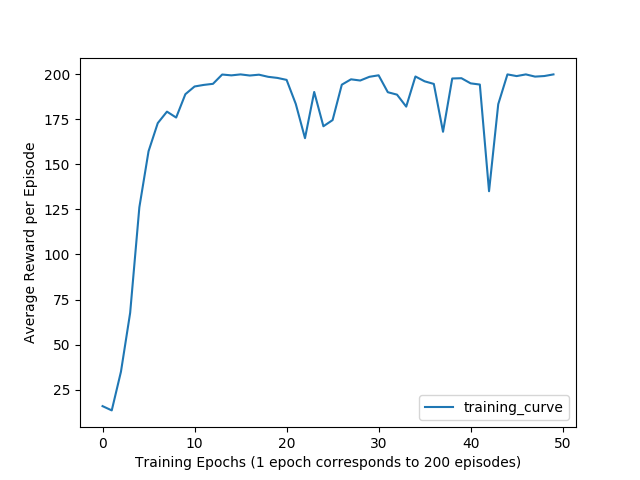
\includegraphics[width=.5\textwidth]{figures/CP_dueling_training_curve}
    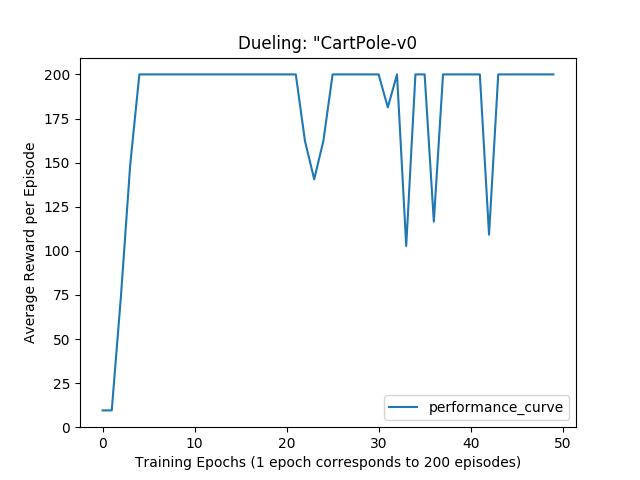
\includegraphics[width=.5\textwidth]{figures/CP_dueling_performance_curve} 
    The training curve for the Dueling network shows sooner convergence on the CP task (around training epoch 10) than the other two Q Network models. We believe the drops in performance after epoch 20 and through epoch 40 could be avoided or subdued with a quicker decay of our epsilon value, as Dueling model converged much sooner than the epsilon decayed to its minimal value.  The performance curve for the Dueling network is not as stable as that of the DDQN network after ~25 training epochs, which may be due again to the differing epsilon decay rates and the fact that the DDQN model ran a minibatch update 4x's as often as the Dueling network. and could therefore have learned more robustly from its epsilon-greedy policy.\\
    {\large Mountaincar-v0 Dueling training and performace plots:} \\
    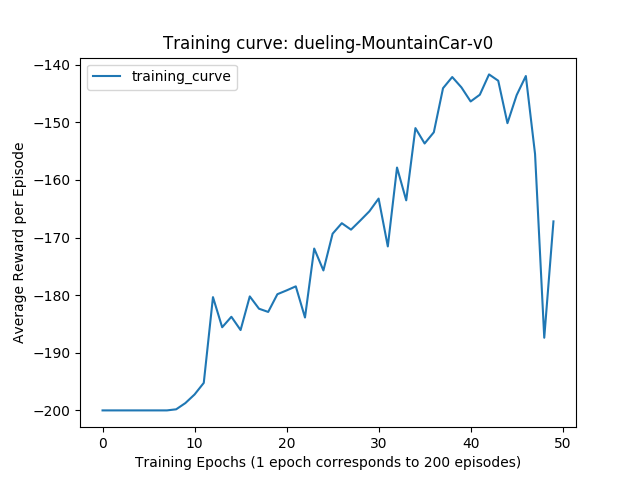
\includegraphics[width=.5\textwidth]{figures/MC_dueling_training_curve}
    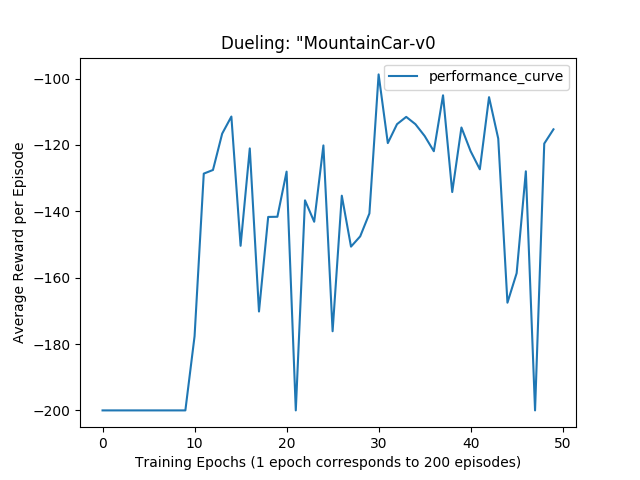
\includegraphics[width=.5\textwidth]{figures/MC_dueling_performance_curve}\\ 
    The MC environment was quite difficult for the Dueling network. Hyperparameters tuned included the width of the 2 network streams and the number of shared layers, epsilon decay rate, learning rate, and optimizer. Also, we experimented with a hyperparameter included in the Atari DQN paper (arXiv), which was the number of frames skipped/over which to repeat previous actions. Ultimately, the best performing instance of the model could reach the goal consistently after episode returns above -200 (i.e. rewarding it in the range of [-80, -190]) after only 10 training epochs. This is almost a factor of 3 times sooner than the other networks for this task. According to the performance plot, the Dueling network outperforms the DQN and DDQN from epoch 10 until it is overtaken around epoch 35 by both DQN and DDQN. The Dueling netowkr's performance curve also shows the most variance in its non-(-200) episode reward compared to the other networks, and we believe this could be improved with a smaller learning rate and by updating the target network ($\theta^{-}$, from DQN) more comparably often to the other networks in order to induce greatly stability in the loss as a function of the training epochs. In the end, the Dueling network outperformed in terms of convergence rate, but for the summary statistics in Table 30, it appears its high episodic return variance was a detriment. The other networks had smaller mean reward and smaller standard deviation for the test episodes.\\
    {\large 6.3 (d):} please refer to the submitted videos. \\
    {\large 6.3 (e):} The below table was generated using a \textbf{greedy} policy.
        \begin{table}[H]
    	\centering
    	\caption{ Dueling:  Avg. total reward per 100 episode +/- std.}
    	\begin{tabular}{|p{9.43em}|r|}
    		\hline
    		\textbf{\small Setting} & \multicolumn{1}{p{10.645em}|}{\textbf{ \small mean $\pm$ std.}} \\
    		\hline
    		{\small CartPole Dueling} & \multicolumn{1}{l|}{\footnotesize 200.0 $\pm$ 0.0}  \\
    		\hline
    		{\small MountainCar Dueling} & \multicolumn{1}{l|}{\footnotesize -133.01 $\pm$ 27.5672} \\
    		\hline
    	\end{tabular}%
    	\label{tab4}%
    \end{table}%
    \end{tcolorbox}
    \begin{tcolorbox}[fit,height=22cm, width=\textwidth, blank, borderline={1pt}{-2pt},nobeforeafter]
        \begin{table}[H]
    	\centering
    	\caption{ Summary: Avg. total reward per 100 episode +/- std.}
    	\begin{tabular}{|p{9.43em}|r|}
    		\hline
    		\textbf{\small Setting} & \multicolumn{1}{p{10.645em}|}{\textbf{ \small mean $\pm$ std.}} \\
    		\hline
    		{\small CartPole DQN} & \multicolumn{1}{l|}{200.0 $\pm$ 0.0} \\
    		\hline
    		{\small CartPole DQN} \newline{} {\small(2 step look ahead)} & \multicolumn{1}{l|}{200.0 $\pm$ 0.0} \\
    		\hline
    		{\small CartPole DDQN} & \multicolumn{1}{l|}{200.0 $\pm$ 0.0} \\
    		\hline
    		{\small CartPole Dueling} & \multicolumn{1}{l|}{200.0 $\pm$ 0.0} \\
    		\hline
    		{\small MountainCar DQN} & \multicolumn{1}{l|}{-109.85 $\pm$ 11.6115} \\
    		\hline
    		{\small MountainCar DDQN} & \multicolumn{1}{l|}{-108.59 $\pm$ 9.8347} \\
    		\hline
    		{\small MountainCar Dueling} & \multicolumn{1}{l|}{-133.01 $\pm$ 27.5672} \\
    		\hline
    	\end{tabular}%
    	\label{tab5}%
    \end{table}%
    \end{tcolorbox}
\end{document}
